%%%%%%%%%%%%%%%%%%%%%%%%%%%%%%%%%%%%%%%%%%%%%%%%%%%%%%%%%%%%%%%%%%%%%%
% LaTeX Template: Curriculum Vitae
%
% Source: http://www.howtotex.com/
% Feel free to distribute this template, but please keep the
% referal to HowToTeX.com.
% Date: July 2011
% 
%%%%%%%%%%%%%%%%%%%%%%%%%%%%%%%%%%%%%%%%%%%%%%%%%%%%%%%%%%%%%%%%%%%%%%
% How to use writeLaTeX: 
%
% You edit the source code here on the left, and the preview on the
% right shows you the result within a few seconds.
%
% Bookmark this page and share the URL with your co-authors. They can
% edit at the same time!
%
% You can upload figures, bibliographies, custom classes and
% styles using the files menu.
%
% If you're new to LaTeX, the wikibook is a great place to start:
% http://en.wikibooks.org/wiki/LaTeX
%
%%%%%%%%%%%%%%%%%%%%%%%%%%%%%%%%%%%%%%%%%%%%%%%%%%%%%%%%%%%%%%%%%%%%%%
\documentclass[paper=a4,fontsize=11pt]{scrartcl} % KOMA-article class
							
\usepackage[english]{babel}
\usepackage[utf8x]{inputenc}
\usepackage[protrusion=true,expansion=true]{microtype}
\usepackage{amsmath,amsfonts,amsthm}     % Math packages
\usepackage{graphicx}                    % Enable pdflatex
\usepackage[svgnames]{xcolor}            % Colors by their 'svgnames'
\usepackage{geometry}
	\textheight=700px                    % Saving trees ;-)
\usepackage{url}

\frenchspacing              % Better looking spacings after periods
\pagestyle{empty}           % No pagenumbers/headers/footers

%%% Custom sectioning (sectsty package)
%%% ------------------------------------------------------------
\usepackage{sectsty}

\sectionfont{%			            % Change font of \section command
	\usefont{OT1}{phv}{b}{n}%		% bch-b-n: CharterBT-Bold font
	\sectionrule{0pt}{0pt}{-5pt}{3pt}}

%%% Macros
%%% ------------------------------------------------------------
\newlength{\spacebox}
\settowidth{\spacebox}{8888888888}			% Box to align text
\newcommand{\sepspace}{\vspace*{1em}}		% Vertical space macro

\newcommand{\MyName}[1]{ % Name
		\Huge \usefont{OT1}{phv}{b}{n} \hfill #1
		\par \normalsize \normalfont}
		
\newcommand{\MySlogan}[1]{ % Slogan (optional)
		\large \usefont{OT1}{phv}{m}{n}\hfill \textit{#1}
		\par \normalsize \normalfont}

\newcommand{\NewPart}[1]{\section*{\uppercase{#1}}}

\newcommand{\PersonalEntry}[2]{
		\noindent\hangindent=2em\hangafter=0 % Indentation
		\parbox{\spacebox}{        % Box to align text
		\textit{#1}}		       % Entry name (birth, address, etc.)
		\hspace{1.5em} #2 \par}    % Entry value

\newcommand{\SkillsEntry}[2]{      % Same as \PersonalEntry
		\noindent\hangindent=2em\hangafter=0 % Indentation
		\parbox{\spacebox}{        % Box to align text
		\textit{#1}}			   % Entry name (birth, address, etc.)
		\hspace{1.5em} #2 \par}    % Entry value	
		
\newcommand{\EducationEntry}[4]{
		\noindent \textbf{#1} \hfill      % Study
		\colorbox{Black}{%
			\parbox{6em}{%
			\hfill\color{White}#2}} \par  % Duration
		\noindent \textit{#3} \par        % School
		\noindent\hangindent=2em\hangafter=0 \small #4 % Description
		\normalsize \par}

\newcommand{\WorkEntry}[4]{				  % Same as \EducationEntry
		\noindent \textbf{#1} \hfill      % Jobname
		\colorbox{Black}{\color{White}#2} \par  % Duration
		\noindent \textit{#3} \par              % Company
		\noindent\hangindent=2em\hangafter=0 \small #4 % Description
		\normalsize \par}

%%% Begin Document
%%% ------------------------------------------------------------
\begin{document}
% you can upload a photo and include it here...
%\begin{wrapfigure}{l}{0.5\textwidth}
%	\vspace*{-2em}
%		
\includegraphics[width=0.15\textwidth]{photo}
%\end{wrapfigure}
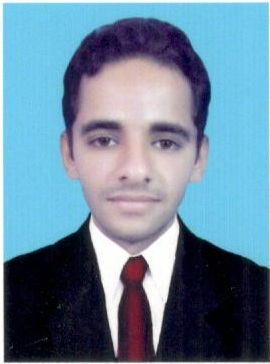
\includegraphics[width=0.2\textwidth]{pic_bof_khan_g.jpeg}

\MyName{Khizar Hayat}
\MySlogan{Curriculum Vitae}



%%% Personal details
%%% ------------------------------------------------------------
\NewPart{Personal details}{}

\PersonalEntry{Birth}{April 15, 1995}
\PersonalEntry{Address}{Chah Dadan Walla Chak No 125/TDA Tehsil and District Layyah}
\PersonalEntry{Phone}{(+92) 305-7381506 (+92-335-7787831) }
\PersonalEntry{Mail}{\url{khizarbhullar59@gmail.com}}
\PersonalEntry{CNIC NO}{32203-1585984-1}
\PersonalEntry{Religion}{Islam}
\PersonalEntry{Nationality}{Pakistani}
\PersonalEntry{Domicile}{Layyah(Punjab)}
\PersonalEntry{Marital Status} {Single}

%%% Education
%%% ------------------------------------------------------------
\NewPart{Education}{}

\EducationEntry{B.SC Engineering and Technology}{2013-2017}{Government College University Faisalabad Layyah Campus}{CGPA}
 {3.62/4.00}



\EducationEntry{DAE(Diploma of Associate Engineer
)}{2010-2013}{Government College Of Technology Layyah}{2876/3550}
{81\%}


\EducationEntry{Matriculation}{2009-2010}{Punjab Islamia Public School Layyah}{733/1050}
\newpage

%%% Work experience
%%% ------------------------------------------------------------
\NewPart{Work experience}{}

\EducationEntry{Prime Minister Youth Internship Program}{2016-2017}{Government College Of Technology Layyah}{One Year Internship (Prime Minister Youth Internship Program)(July 2016-July 2017) for the purpose of improving the technical skills(tracking ID(111040))}


\EducationEntry{MEPCO Training}{08-07-2013-08-08-2013}{Multan Electric Power Company Multan}{Completed his internship training from 08-07-2013 to 08-08-2013 in electrical training from 132KV grid station MEPCO layyah.}

%%% Skills
%%% ------------------------------------------------------------
\NewPart{Skills}{}

\SkillsEntry{Languages}{English}
\SkillsEntry{}{Urdu}
\SkillsEntry{}{Saraiki}

\SkillsEntry{Engineering Software}{\textsc{Matlab}, \LaTeX, \textsc{Multisim}, \textsc{proteus},\textsc{workbench},\textsc{PCPIS},\textsc{Keil} }
\SkillsEntry{Additional software}{\textsc{Microsoft office(MS word,power point)}}
%%% Skills
%%% ------------------------------------------------------------
\NewPart{hobbies}{work on software and web design,\\playing cricket}
%%% Skills
%%% ------------------------------------------------------------
\NewPart{Reference}{Will be provided on demand. }
\end{document}
